\section{Methodology}
\label{sec:methodology}

This section provides the details of the implementation of the empirical process. At a high level, two experimental groups are executed. These include a behavioural case study and a comparison between the \acs{BHH} and standalone low-level heuristics. A number of datasets, models and heuristics are specified. Throughout the empirical process, the use of a \acs{BHH} baseline configuration is used.

\subsection{BHH Baseline}\label{sec:methodology:baseline_bhh}

The \acs{BHH} baseline is a name given to a specific configuration of the \acs{BHH} which has been found to provide a reasonable baseline performance. The baseline configuration is used as the cornerstone configuration from which all other heuristics and their configurations are evaluated. The \acs{BHH} baseline configuration is given in Table \ref{tab:methodology:bhh_baseline_configuration}. In Table \ref{tab:methodology:bhh_baseline_configuration}, the heuristic pool configuration, \textit{all}, refers to a configuration where the heuristic pool contains all the low-level heuristics, including all gradient-based heuristics and \acp{MH}.

% Table generated by Excel2LaTeX from sheet 'BHH Baseline'
\begin{table}[htb]
	\centering
	\caption{The \acs{BHH} baseline configuration as it is used in the empirical study.}
	\label{tab:methodology:bhh_baseline_configuration}%
	\par\bigskip
	\resizebox{0.70\textwidth}{!}{
		\begin{tabular}{rrcc}
			\multicolumn{1}{c}{\textbf{hyper-heuristic}} & \multicolumn{1}{c}{\textbf{variant}} & \textbf{configuration} & \textbf{value} \\
			\midrule
			\multicolumn{1}{l}{bhh}                      & \multicolumn{1}{l}{baseline}         & heuristic pool         & all            \\
			                                             &                                      & population             & 5              \\
			                                             &                                      & credit                 & ibest          \\
			                                             &                                      & burn in                & 0              \\
			                                             &                                      & reselection            & 10             \\
			                                             &                                      & replay                 & 10             \\
			                                             &                                      & reanalysis             & 10             \\
			                                             &                                      & normalise              & false          \\
			                                             &                                      & discounted rewards     & false          \\
		\end{tabular}%
	}
\end{table}%


\subsection{Experiments}
\label{sec:methodology:experiments}

This section provides the details of the two experimental groups that are implemented and executed.

\subsubsection{Behavioural Case Study}
\label{sec:methodology:experiments:case_study}

The behavioural case study analyses the behaviour of the \acs{BHH} baseline configuration as it relates to an example problem dataset. The example problem dataset is the iris dataset, presented in Table \ref{tab:methodology:datasets:classification}. The behavioural case study provides insight into the inner workings of the \acs{BHH}. The \acs{BHH} baseline, by default, has a replay window size of 10. The baseline configuration is compared to an implementation of a \acs{BHH} configuration where the replay window size is large (250), as well as an implementation of the \acs{BHH} using the \textit{symmetric} credit assignment strategy. The large replay window size configuration is used to show the behaviour of the \acs{BHH} when it has access to a large number of performance log samples, which increases the statistical certainty of the learning outcome. The \acs{BHH} configuration that uses the \textit{symmetric} credit assignment strategy is used to illustrate the behaviour of the \acs{BHH} where no performance bias takes place and thus, no learning occurs.

\subsection{Standalone Heuristics}
\label{sec:methodology:experiments:standalone_optimisers}

For the standalone heuristics experimental group, a number of low-level heuristics are used along with their specified hyper-parameters. Each of these standalone low-level heuristics are compared to that of the \acs{BHH} baseline configuration, across all datasets. The intent of the standalone heuristics experimental group is to determine if the \acs{BHH} baseline configuration can generalise to multiple problems in comparison to individual low-level heuristics.

Additional to the \acs{BHH} baseline configuration, two more \acs{BHH} configurations are included. These include \acs{BHH} configurations where the heuristic pool only makes use of gradient-based heuristics, and a configuration where the heuristic pool only makes use of \acp{MH}. The intent behind the inclusion of these configurations is to determine the effectiveness of multi-method approaches in the heuristic pool as it applies to training \acp{FFNN}.

\subsection{Heuristics}\label{sec:methodology:heuristics}

Table \ref{tab:methodology:heuristics} contains a list of all the standalone, low-level heuristics that are used as well as their hyper-parameter configurations. Note from Table \ref{tab:methodology:heuristics} that values that are configured to make use of a decay schedule are presented with the initial value first and the decay rate in brackets next to it.


\begin{table}[htbp]
	\centering
	\caption{Low-level heuristics and their hyper-parameter configurations.}
	\label{tab:methodology:heuristics}%
	\par\bigskip
	\resizebox{0.7\textwidth}{!}{

		\begin{tabular}{llll}
			\textbf{heuristic} & \textbf{configuration}    & \textbf{value} & \textbf{citation}         \\
			\midrule
			sgd                & learning rate             & 0.1 (0.01)     & \cite{ref:sutskever:2013} \\
			momentum           & learning rate             & 0.1 (0.01)     & \cite{ref:sutskever:2013} \\
			                   & momentum                  & 0.9            &                           \\
			nag                & learning rate             & 0.1 (0.01)     & \cite{ref:sutskever:2013} \\
			                   & momentum                  & 0.9            &                           \\
			adagrad            & learning rate             & 0.1 (0.01)     & \cite{ref:duchi:2011}     \\
			                   & epsilon                   & 1E-07          &                           \\
			rmsprop            & learning rate             & 0.1 (0.01)     & \cite{ref:hinton:2012}    \\
			                   & rho                       & 0.95           &                           \\
			                   & epsilon                   & 1E-07          &                           \\
			adadelta           & learning rate             & 1.0 (0.95)     & \cite{ref:zeiler:2012}    \\
			                   & rho                       & 0.95           &                           \\
			                   & epsilon                   & 1E-07          &                           \\
			adam               & learning rate             & 0.1 (0.01)     & \cite{ref:kingma:2014}    \\
			                   & beta1                     & 0.9            &                           \\
			                   & beta2                     & 0.999          &                           \\
			                   & epsilon                   & 1E-07          &                           \\
			pso                & population size           & 10             & \cite{ref:van:2010}       \\
			                   & learning rate             & 1.0 (0.9)      &                           \\
			                   & inertia weight (w)        & 0.729844       &                           \\
			                   & cognitive control (c1)    & 1.49618        &                           \\
			                   & social control (c2)       & 1.49618        &                           \\
			                   & velocity clip min         & -1.0           &                           \\
			                   & velocity clip max         & 1.0            &                           \\
			de                 & population size           & 10             & \cite{ref:mezura:2006}    \\
			                   & selection strategy        & best           &                           \\
			                   & xo strategy               & exp            &                           \\
			                   & recombination probability & 0.9 (0.1)      &                           \\
			                   & beta                      & 2.0 (0.1)      &                           \\
			ga                 & population size           & 10             & \cite{ref:lambora:2019}   \\
			                   & selection strategy        & rand           &                           \\
			                   & xo strategy               & bin            &                           \\
			                   & mutation rate             & 0.2 (0.05)     &                           \\
		\end{tabular}%
	}
\end{table}%


The mapping of proxied heuristic state update operations implemented by the \acs{BHH} in the empirical process is given in Figure \ref{fig:methodology:heuristics:proxies}. In Figure \ref{fig:methodology:heuristics:proxies}, cells containing \textbf{x} indicate that the associated heuristic implements that particular state parameter explicitly, and cells containing \textbf{o} indicate that the state parameter is implicitly implemented as part of the \acs{BHH} algorithm.

\begin{figure}[htbp]
	\centering
	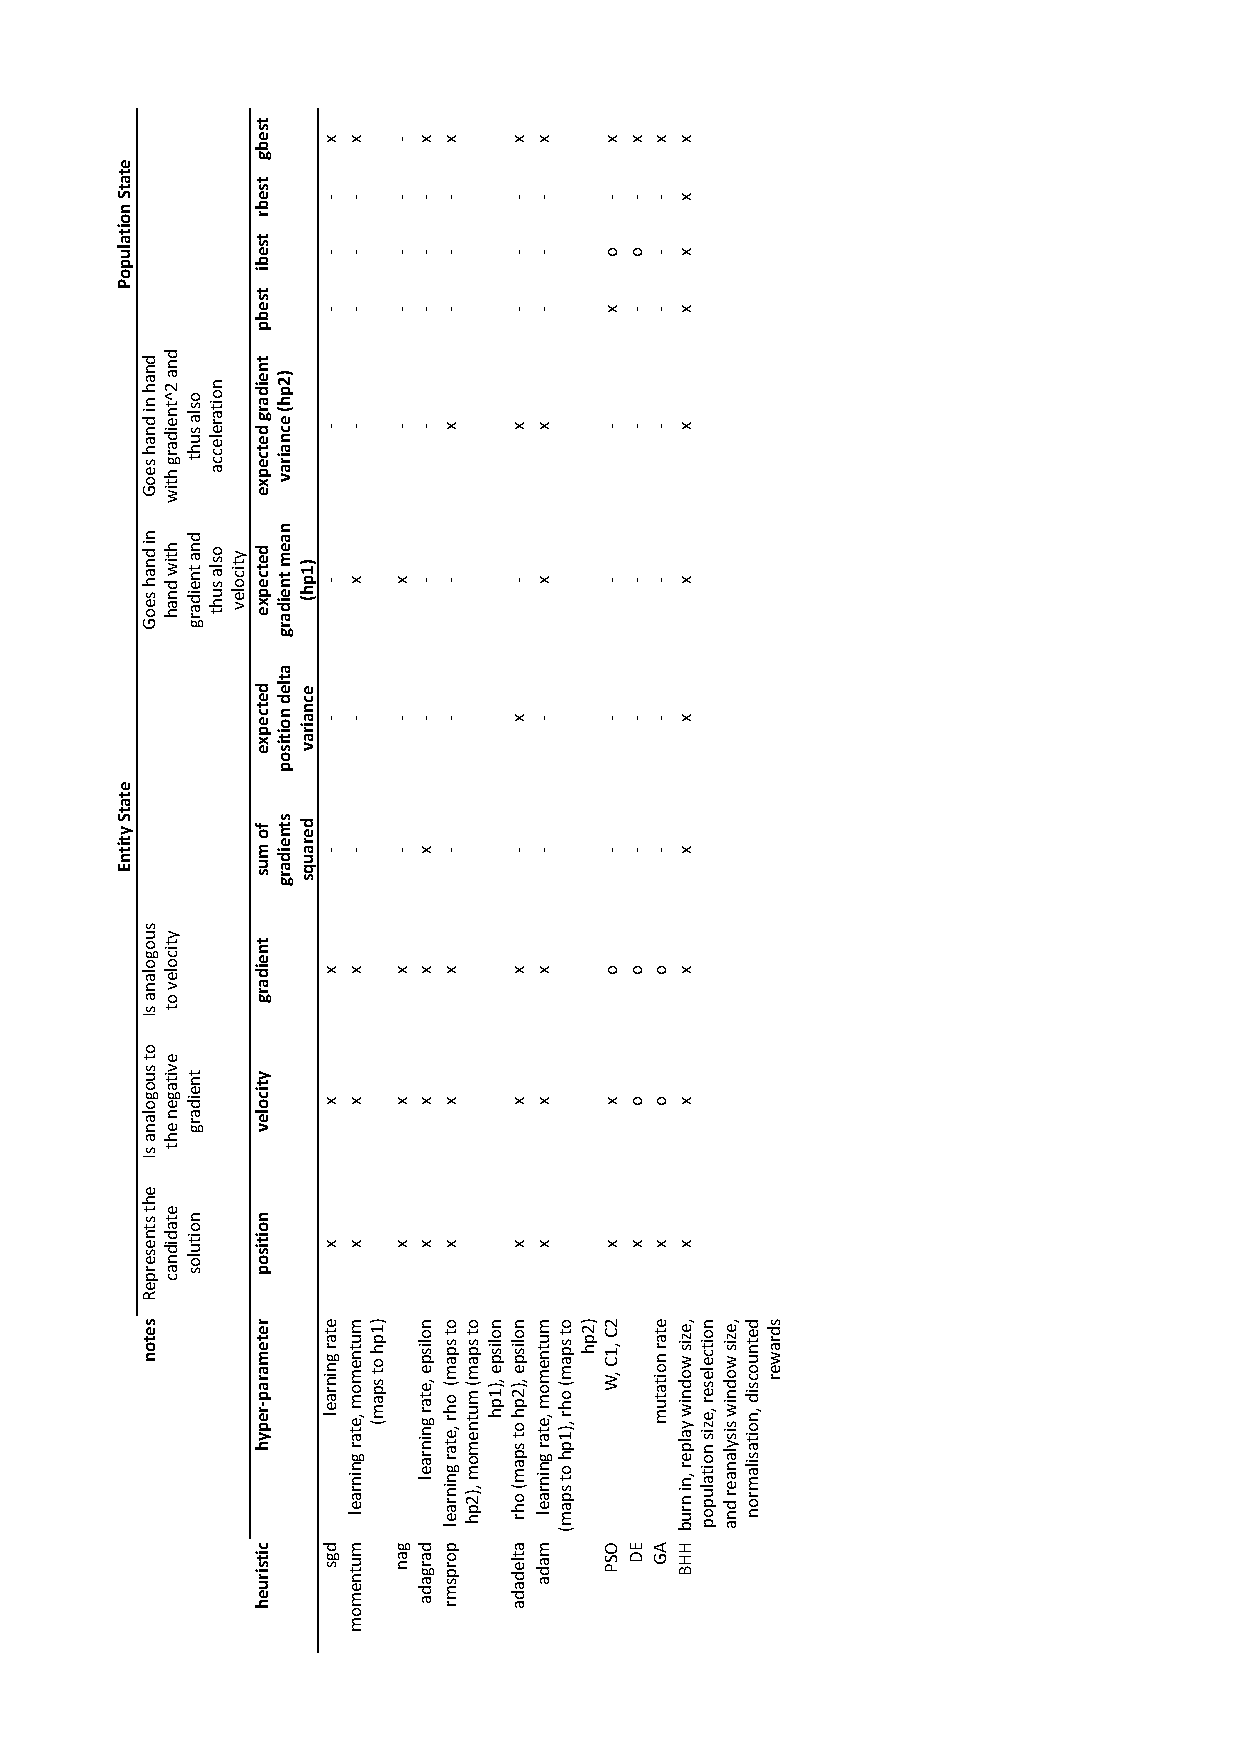
\includegraphics[width=0.8\textwidth]{images/bhh_heuristic_proxies.pdf}
	\caption{Mapping of proxied heuristic state update operations as implemented by the \acs{BHH}}
	\label{fig:methodology:heuristics:proxies}%
\end{figure}


\subsection{Datasets}\label{sec:methodology:datasets}

In the context of training \acp{FFNN}, the underlying models are trained across a number of datasets. All the datasets used in the empirical process originate from the UCI Machine Learning Repository \cite{ref:uci:2022}. Datasets are grouped by problem type and include seven classification and seven regression datasets. The details around the datasets used can be found in Tables \ref{tab:methodology:datasets:classification} and \ref{tab:methodology:datasets:regression}. Each dataset is split into a training set comprising of 80\% of the data, and a test set comprising of 20\% of the data. The test set is used as a validation set during training.

A number of classification datasets contain an unbalanced representation of classes. This work does not apply mechanisms to cater for class balancing, in order to eliminate as many variables and factors in the empirical process as possible.


\begin{table}[htb]
	\centering
	\caption{Classification datasets}
	\label{tab:methodology:datasets:classification}%
	\par\bigskip
	\resizebox{\textwidth}{!}{
		\begin{tabular}{ccccccccc}
			\textbf{dataset} & \textbf{output} & \textbf{types}             & \textbf{attributes} & \textbf{classes} & \textbf{instances} & \textbf{batch} & \textbf{steps} & \textbf{citation}         \\
			\midrule
			iris             & multivariate    & real                       & 4                   & 3                & 150                & 16             & 10             & \cite{ref:fisher:1936}    \\
			car              & multivariate    & categorical                & 6                   & 4                & 1728               & 128            & 14             & \cite{ref:bohanec:1988}   \\
			abalone          & multivariate    & categorical, integer, real & 8                   & 28               & 4177               & 256            & 17             & \cite{ref:waugh:1995}     \\
			wine quality     & multivariate    & real                       & 12                  & 11               & 4898               & 256            & 20             & \cite{ref:cortez:2009}    \\
			mushroom         & multivariate    & categorical                & 22                  & 2                & 8214               & 512            & 17             & \cite{ref:schlimmer:1987} \\
			bank             & multivariate    & real                       & 17                  & 2                & 45211              & 512            & 89             & \cite{ref:moro:2014}      \\
			diabetic         & multivariate    & integer                    & 55                  & 3                & 100000             & 1024           & 98             & \cite{ref:strack:2014}    \\
		\end{tabular}%
	}
\end{table}%

\begin{table}[htb]
	\centering
	\caption{Regression datasets}
	\label{tab:methodology:datasets:regression}%
	\par\bigskip
	\resizebox{\textwidth}{!}{
		\begin{tabular}{cccccccc}
			\textbf{dataset}    & \textbf{output}           & \textbf{types} & \textbf{attributes} & \textbf{instances} & \textbf{batch} & \textbf{steps} & \textbf{citation}        \\
			\midrule
			fish toxicity       & multivariate              & real           & 7                   & 908                & 64             & 15             & \cite{ref:cassotti:2015} \\
			housing             & univariate                & real           & 13                  & 506                & 32             & 16             & \cite{ref:harrison:1978} \\
			forest fires        & multivariate              & real           & 13                  & 517                & 32             & 17             & \cite{ref:cortez:2007}   \\
			student performance & multivariate              & integer        & 33                  & 649                & 32             & 21             & \cite{ref:cortez:2008}   \\
			parkinsons          & multivariate              & integer, real  & 26                  & 5875               & 256            & 23             & \cite{ref:tsanas:2009}   \\
			air quality         & multivariate, time series & real           & 15                  & 9358               & 256            & 37             & \cite{ref:de:2008}       \\
			bike                & univariate                & integer, real  & 16                  & 17389              & 256            & 68             & \cite{ref:fanaee:2014}   \\
		\end{tabular}%
	}
\end{table}%

\subsection{Models}\label{sec:methodology:model}

All models that are trained in the empirical process follow implementations of shallow \acp{FFNN} with only one hidden layer. The number of hidden units used were determined empirically. Weights are initialised by means of \textit{Glorot uniform sampling} \cite{ref:glorot:2010}. The models and their configuration, as it is used for each dataset, are given in Table \ref{tab:methodology:models:configurations}.


\begin{table}[htb]
	\centering
	\caption{Model configurations}
	\label{tab:methodology:models:configurations}%
	\par\bigskip
	\resizebox{\textwidth}{!}{
		\begin{tabular}{rcccccccc}
			\textbf{dataset}    & \textbf{inputs} & \textbf{hidden} & \textbf{output} & \textbf{biases} & \textbf{parameters} & \textbf{topology} & \textbf{l1 activation} & \textbf{l2 activation} \\
			\midrule
			fish toxicity       & 6               & 3               & 1               & yes             & 25                  & dense             & LReLU ($\alpha = 0.3$) & sigmoid                \\
			iris                & 4               & 5               & 3               & yes             & 43                  & dense             & LReLU ($\alpha = 0.3$) & softmax                \\
			air quality         & 12              & 8               & 1               & yes             & 113                 & dense             & LReLU ($\alpha = 0.3$) & sigmoid                \\
			housing             & 13              & 8               & 1               & yes             & 121                 & dense             & LReLU ($\alpha = 0.3$) & sigmoid                \\
			wine quality        & 13              & 10              & 7               & yes             & 217                 & dense             & LReLU ($\alpha = 0.3$) & softmax                \\
			parkinsons          & 21              & 10              & 1               & yes             & 231                 & dense             & LReLU ($\alpha = 0.3$) & sigmoid                \\
			car                 & 21              & 10              & 4               & yes             & 264                 & dense             & LReLU ($\alpha = 0.3$) & softmax                \\
			forest fires        & 43              & 16              & 1               & yes             & 721                 & dense             & LReLU ($\alpha = 0.3$) & sigmoid                \\
			abalone             & 10              & 36              & 28              & yes             & 1432                & dense             & LReLU ($\alpha = 0.3$) & softmax                \\
			bank                & 51              & 32              & 1               & yes             & 1697                & dense             & LReLU ($\alpha = 0.3$) & softmax                \\
			bike                & 61              & 32              & 1               & yes             & 2017                & dense             & LReLU ($\alpha = 0.3$) & sigmoid                \\
			student performance & 99              & 32              & 1               & yes             & 3233                & dense             & LReLU ($\alpha = 0.3$) & sigmoid                \\
			adult               & 108             & 64              & 1               & yes             & 7041                & dense             & LReLU ($\alpha = 0.3$) & softmax                \\
			mushroom            & 117             & 64              & 1               & yes             & 7617                & dense             & LReLU ($\alpha = 0.3$) & softmax                \\
			diabetic            & 2369            & 32              & 3               & yes             & 75939               & dense             & LReLU ($\alpha = 0.3$) & softmax                \\
		\end{tabular}%
	}
\end{table}%


\subsection{Performance Measures}\label{sec:methodology:performance_measures}

\Acf{BinXE} is used for classification problems with two classes and \acf{SparseCatXE} is used for classification problems with more than two classes. For the classification problems, accuracy is also measured. For regression problems, the \acf{MSE} is used as a performance metric. After training has been completed, the \textit{average rank}, based on test loss, for all configurations, is calculated at each mini-batch step.


\subsection{Statistical Analysis}
\label{sec:methodology:statistical_analysis}

Each experiment and configuration is trained for a maximum of 30 epochs and is repeated over 30 independent runs, for each of the applicable datasets. No early-stopping mechanism is used. Statistical analysis is executed on the results from the test datasets. An average rank is calculated across all 30 runs, for both experimental groups and configurations, at each step, for every epoch of training.

The Shapiro-Wilk test for normality \cite{ref:shapiro:1965} ($\alpha$ = 0.001) is used to determine if the results are normally distributed. The Levene's test for equality of variance \cite{ref:levene:1961} ($\alpha$ = 0.001) is used. For experiments with three or more configurations, the \acs{ANOVA} statistical test \cite{ref:fisher:1921} ($\alpha$ = 0.001) is used. The Kruskal-Wallis ranked non-parametric test \cite{ref:kruskal:1952} for statistical significance ($\alpha$ = 0.001) is used for cases where data is not normally distributed. Finally, a post-hoc Tukey honest significant difference test \cite{ref:tukey:1949} ($\alpha$ = 0.001) is used from which significant ranking is retrieved. Descriptive and critical difference plots are then retrieved from these results to provide visual aid.

\subsection{Implementation}\label{sec:methodology:implementation}

All implementations are done from first principles in Python 3.9 using Tensorflow 2.7 and Tensorflow Probability 0.15.0. The source code and data for this research is provided and made public at \url{https://github.com/arneschreuder/masters}.